\chapter{Implementation}
In this chapter, the steps involved in turning a theoretical design into a tangible system will be outlined. Since the synthesis chapter dealt with an explanation of the functions of each module and simulations, with a subsequent evaluation of the outcomes, this chapter will focus on the creation of physical hardware setups and reproducing the desired results using lab experiments. As such, each module will be tested independently to validate its function before a larger, more comprehensive experiment is conducted. All figures in this chapter show measurements performed on physical hardware.
\section{Control System}
\begin{figure}[htbp]
	\centering
	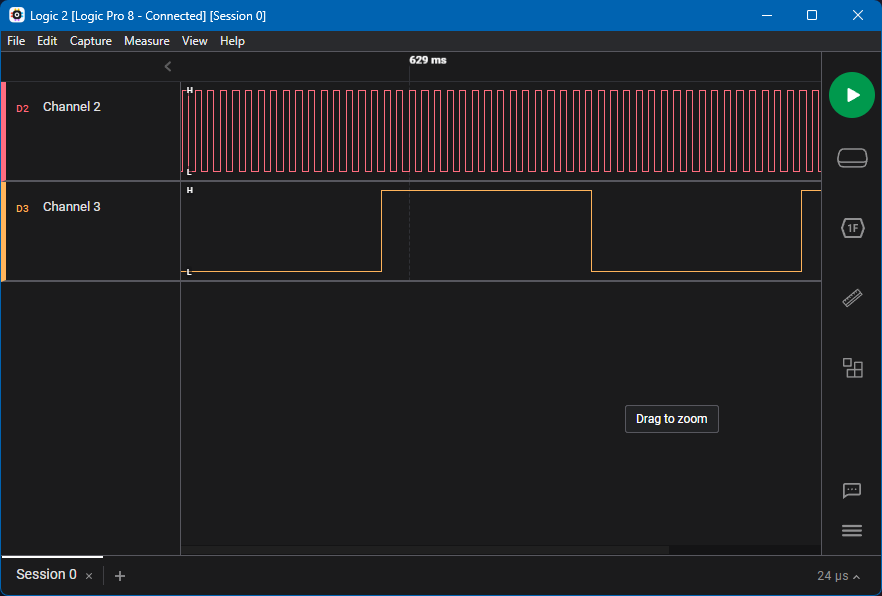
\includegraphics[width=.8\textwidth]{Figures/4_controlsystem_stm32_zephyr.png}
	\caption{STM32 Zephyr RTOS pulser output}
	\label{fig:4_stm32_zephyr_pulser}
\end{figure}
During the initial implementation stage of the control system, a bring-up of the STM32F411RE board and several pulse signals were succesfully generated. In \cref{fig:4_stm32_zephyr_pulser}, two pulse signals can be seen. In Channel 2, \qty{5}{\mega\hertz} ultrasound pulse can be seen. In Channel 3, the \qty{10}{\kilo\hertz} PRF signal can be seen. Unfortunately, soon thereafter it was discovered a limitation of the API in Zephyr is not mature enough developed for power systems such as the half-bridge in the transmitter circuit. In more practical terms, it was not possible to generate two complementary signals with dead-time using the existing Zephyr PWM API. To continue with that solution, a new PWM driver would have to be written from scratch, which is no trivial task. Alternative solutions were investigated. Another option was to use the \gls{hal} provided by the manufacturer of the microcontroller. However, it was decided to try an alternative system known as PYNQ Z1, which is a development board by Agilent. On the PYNQ Z1 board is a Zynq 7000 \gls{soc}. Inside the Zynq 7000 SoC there are both an \gls{fpga} and Arm based processor.

\section{Power Stage}
\begin{figure}[htbp]
	\centering
	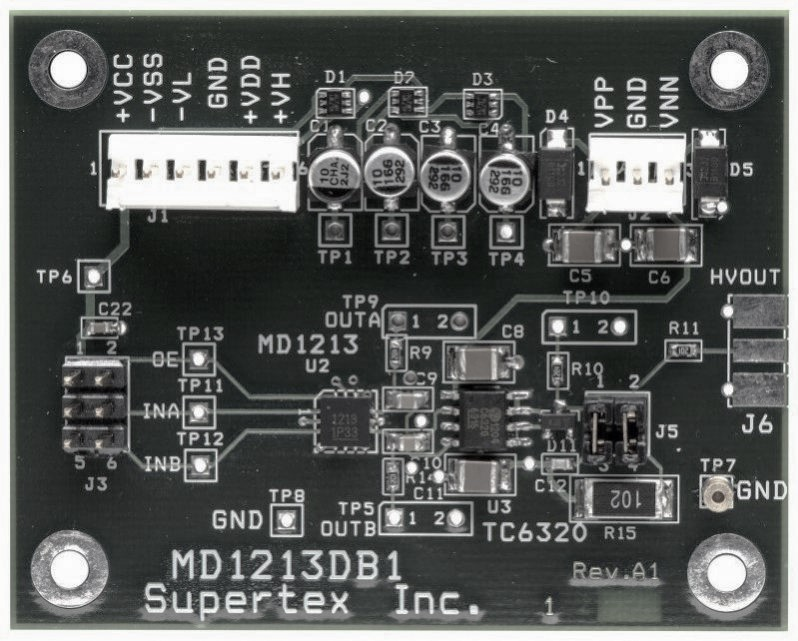
\includegraphics[width=.8\textwidth]{Figures/4_transmitter_pcb_pic.jpg}
	\caption{MD1213DB1 High Speed Pulser}
	\label{fig:4_transmitter_pcb_pic}
\end{figure}
A picture of the power stage PCB can be seen in \cref{fig:4_transmitter_pcb_pic}. An experiment is conducted to validate the function of the power stage. Using the jumpers, the PCB is configured without its onboard load, and a \gls{pzt} transducer is attached with a splitter adapter to connect the other side to an oscilloscope for data acquisition.

\section{Transmit/Receive Switch}
\begin{figure}[htbp]
	\centering
	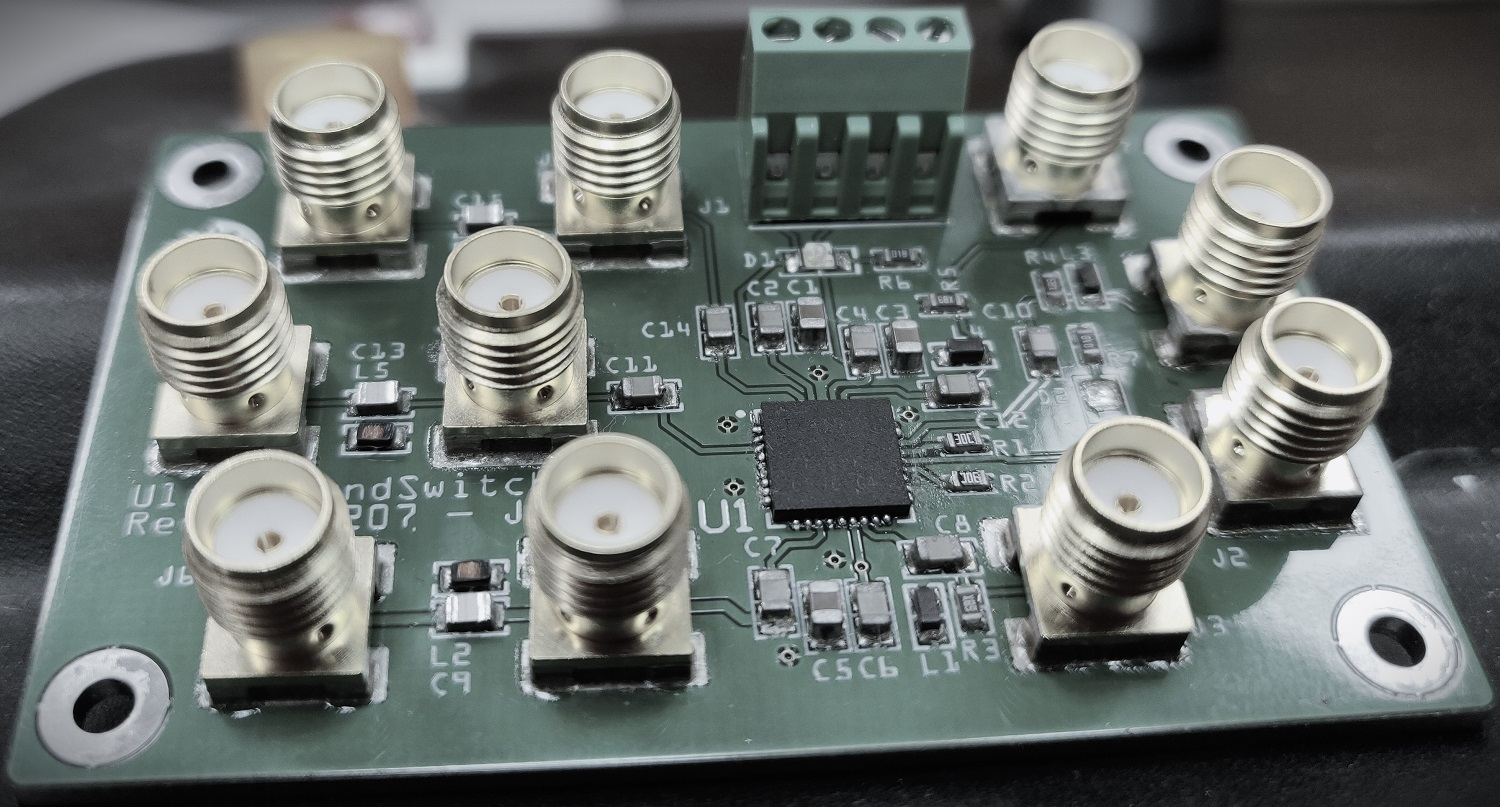
\includegraphics[width=.8\textwidth]{Figures/4_switch_pcb_pic.jpg}
	\caption[Transmit/Receive Switch after assembly]{Transmit/Receive Switch after assembly}
	\label{fig:4_txrx_pcb}
\end{figure}
The entire schematic of the transmit/receive switch can be found in the appendix in \cref{fig:appendix_ultrasoundswitch_a,fig:appendix_ultrasoundswitch_b}. As mentioned in the previous chapter, a PCB layout was made and a batch of 5 was ordered with an accompanying stencil for fast assembly. After the PCBs arrived, the stencil was mounted in the stencil frame and the PCB was aligned for solder paste application. After the solder paste application is completed, all the components are placed on their corresponding footprints and the PCB is placed in the reflow oven. The equipment used in this process is listed in \cref{tab:instruments_solder_work}. The finished assembly can be seen in \cref{fig:4_txrx_pcb}.
\begin{figure}[htbp]
	\centering
	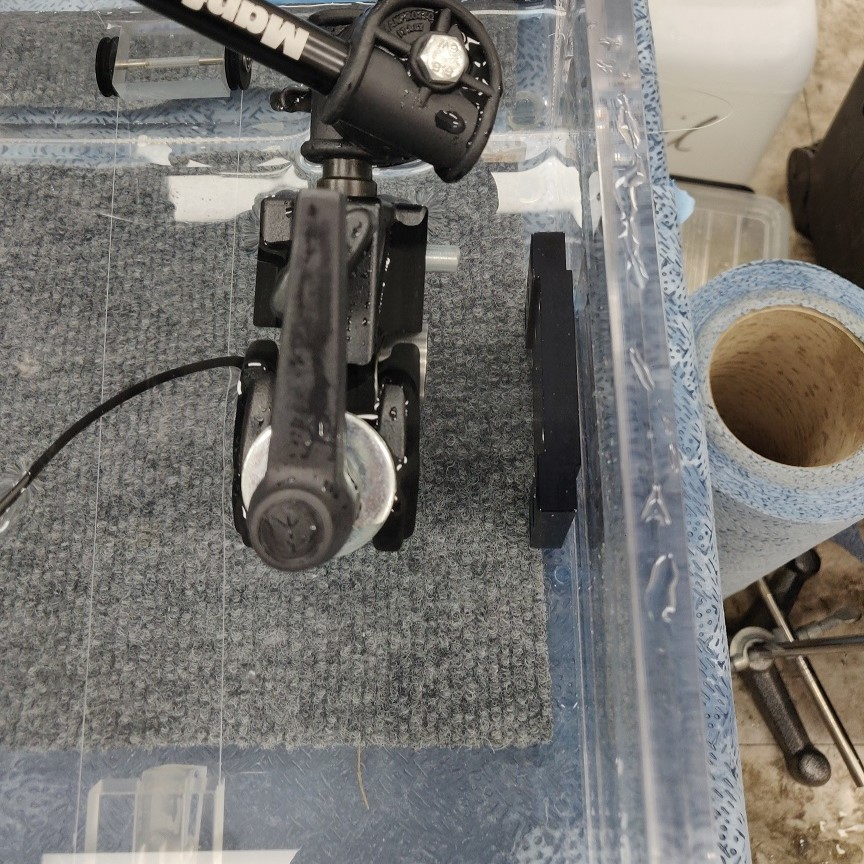
\includegraphics[width=.8\textwidth]{Figures/4_switch_meas_pic.jpg}
	\caption{TX/RX Switch reflection experiment with water tank}
	\label{fig:4_switch_meas_pic}
\end{figure}
For validating the TX/RX switch, an experiment is conducted with a \gls{pzt} transducer, water tank, function generator and an oscilloscope. Using two input signals, $f_{\mathrm{prf}}=\qty{10}{\kilo\hertz}$ switch signal, and $f_{0}=\qty{5}{\mega\hertz}$ burst mode transmit signal, the switch is configured to transmit and receive. A picture of the submerged transducer with a reflector can be seen in \cref{fig:4_switch_meas_pic}. After submerging the transducer in distilled water and measuring on the receiver side of the TX/RX switch, a reflected signal from the tank can be observed in \cref{fig:4_txrx_meas}.
\begin{figure}[htbp]
	\centering
	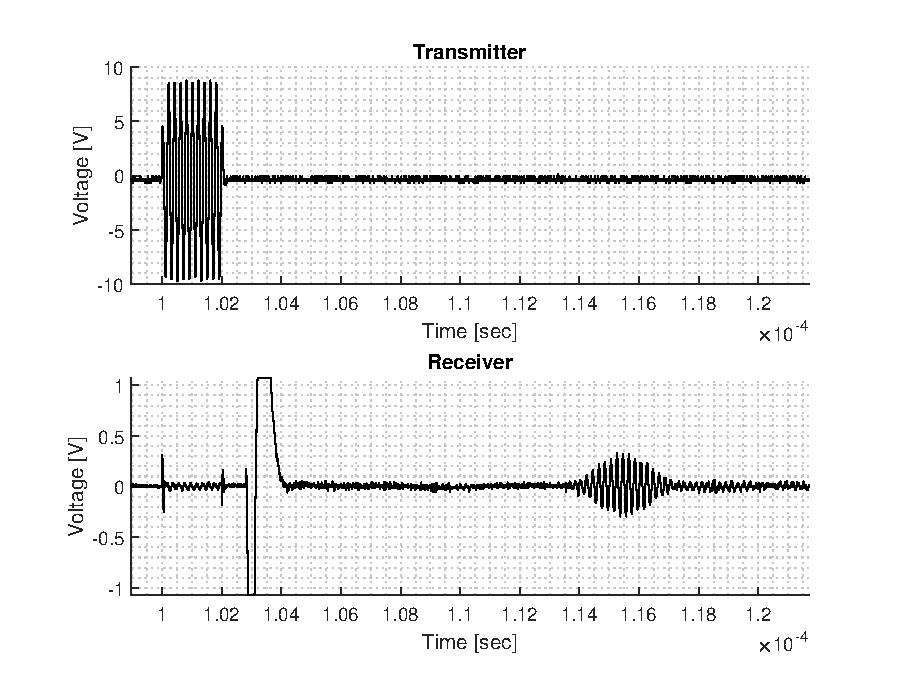
\includegraphics[width=.8\textwidth]{Figures/4_switch_pcb_meas.eps}
	\caption[Measured transmit and receive on Transmit/Receive Switch PCB]{Measured transmit and receive on Transmit/Receive Switch PCB (Above) Measured transmit voltage (Below) Received reflected signal off water tank}
	\label{fig:4_txrx_meas}
\end{figure}
\section{Band-Pass Filter}
As the band-pass filter was described in the previous chapter, it is desired to validate its frequency response to determine if it functions as desired. To obtain the frequency response, a bode plot of the magnitude and phase is measured from \qty{300}{\kilo\hertz} until \qty{20}{\mega\hertz} using a \gls{vna} in a S21 configuration, meaning a measurement of the output in respect to the input. This measurement determines the difference in magnitude and phase of the output in comparison with the input signal. Observed in \cref{fig:4_bpf_measurement} is the frequency response of the band-pass filter measured on a \gls{vna}. It is noted that the pass band frequencies are mostly as expected with \qty{-0.5}{\decibel} frequencies at \qty{1.5}{\mega\hertz} and \qty{7}{\mega\hertz}. Though, the roll-off in the higher stop band appears somewhat lower than in the lower stop band. That would mean that it is plausible that higher frequency noise components are retained in the output than in the lower stop band. For the phase, it seems to have a significant phase delay, going from around \qty{100}{\degree} to \qty{250}{\degree} from the start to the end of the pass band.
\begin{figure}[htbp]
	\centering
	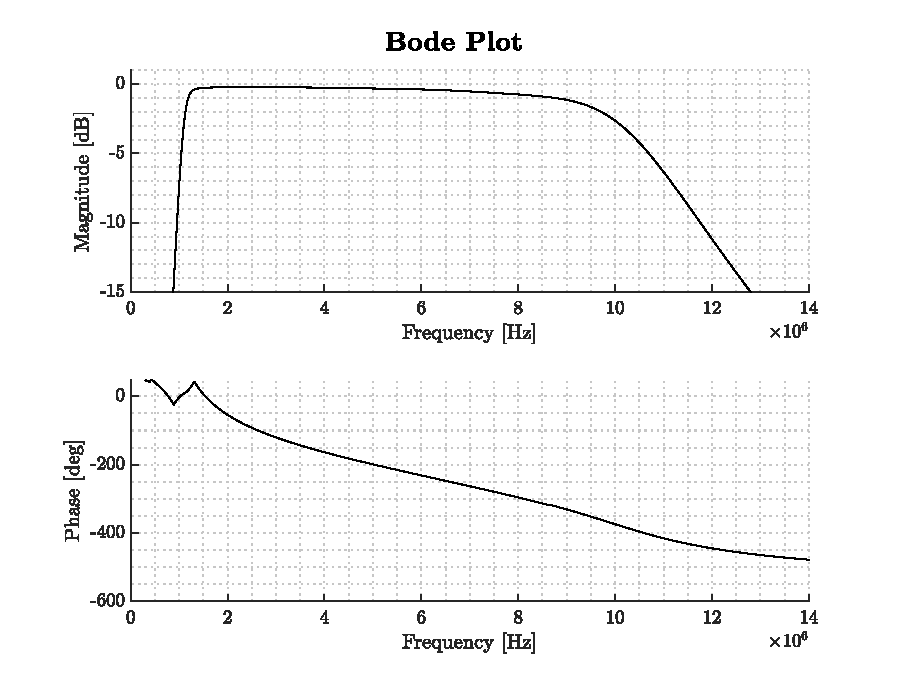
\includegraphics[width=.8\textwidth]{Figures/4_bpf_measurement_vna.eps}
	\caption[Band-pass filter bode plot]{Band-pass Filter bode plot from \qtyrange{0.3}{14}{\mega\hertz} with (above) magnitude and (below) phase}
	\label{fig:4_bpf_measurement}
\end{figure}

\section{Preamplifier}
Before the signal can be demodulated, it must be DC-biased and amplified. This is what the preamplifier is for. For the preamplifier, the circuit is validated using an experiment where a function generator is transmitting a low amplitude sine with ac-coupling and measure the amplified dc-coupled output. Seen in \cref{fig:4_preamp_in} are measurements of the preamplifier circuits showing a \qty{70}{\milli\volt} input signal and a \qty{300}{\milli\volt} output signal with a \qty{2.5}{\volt} DC bias. In this application, however, only the \gls{lna} is used, and the \gls{vga} is bypassed in the hardware preamplifier configuration. The schematic of the preamplifier circuit is part of the demodulation schematic and can be found in the appendix in \cref{fig:appendix_ad8333}.
\begin{figure}[htbp]
	\centering
	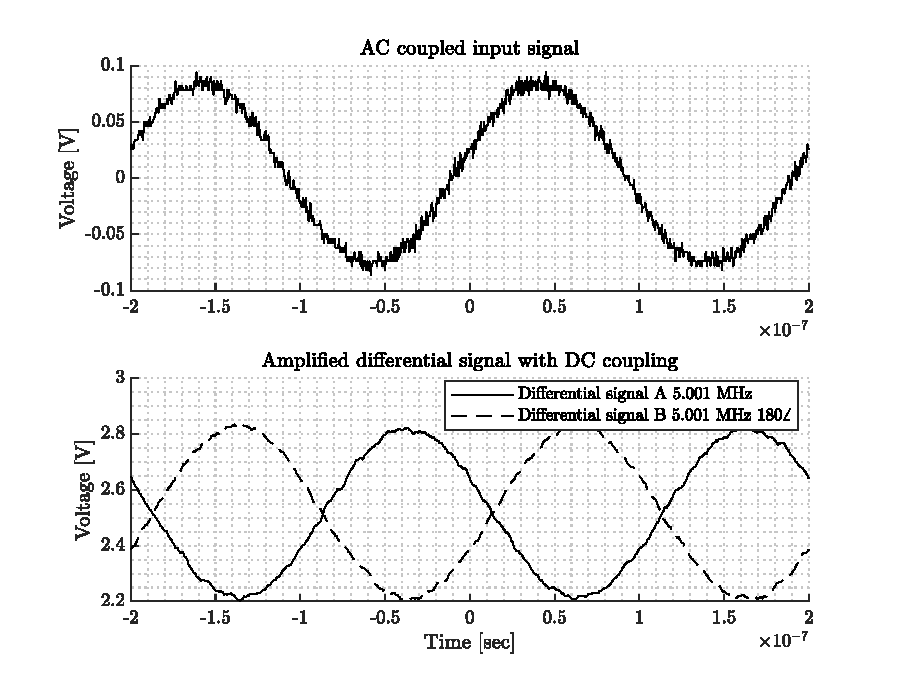
\includegraphics[width=.8\textwidth]{Figures/4_preamplifier_pcb.eps}
	\caption[Measured input and output of preamplifier PCB]{Measured input of preamplifier PCB, (Above) AC coupled input signal with amplitude \qty{1}{\volt} (Below Measured output of preamplifier PCB, Differential signal with DC coupling and $\times \qty{19}{\decibel}$ amplification)}
	\label{fig:4_preamp_in}
\end{figure}
\section{Quadrature Demodulator}
\begin{figure}[htbp]
	\centering
	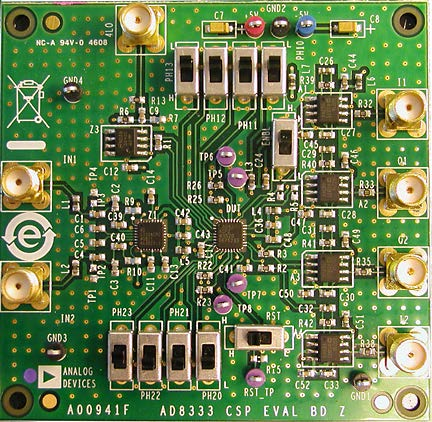
\includegraphics[width=.8\textwidth]{Figures/4_demod_pcb_pic.jpg}
	\caption{Demodulator PCB AD8333-EVALZ}
	\label{fig:4_demod_pcb_pic}
\end{figure}
As described in the previous chapter, the demodulator use an I/Q quadrature demodulation scheme to take two differential RF signals and a quadruple frequency signal, in this case, \qty{5}{\mega\hertz} and \qty{20}{\mega\hertz}, respectively, and determines the frequency difference between the fundamental frequency and the Doppler frequency on the output. Seen in \cref{fig:4_demod_in} are the input signals, differential signals of \qty{5.001}{\mega\hertz} and \qty{20}{\mega\hertz} local oscillator signal. Seen in \cref{fig:4_demod_out} are the differential input signals $A$ and $B$ and the demodulated output signals $I$ and $Q$, where the phase between $I$ and $Q$ denotes the Doppler shift direction, or rather, the direction of flow of the scatterer. It is noted that the differential signal is so high frequency compared to the timescale so there has to be a zoomed in subplot where the waveform is visible to show the waveform. This highlights the significant frequency difference, which is one of the key functions of the demodulator.

\begin{figure}[htbp]
	\centering
	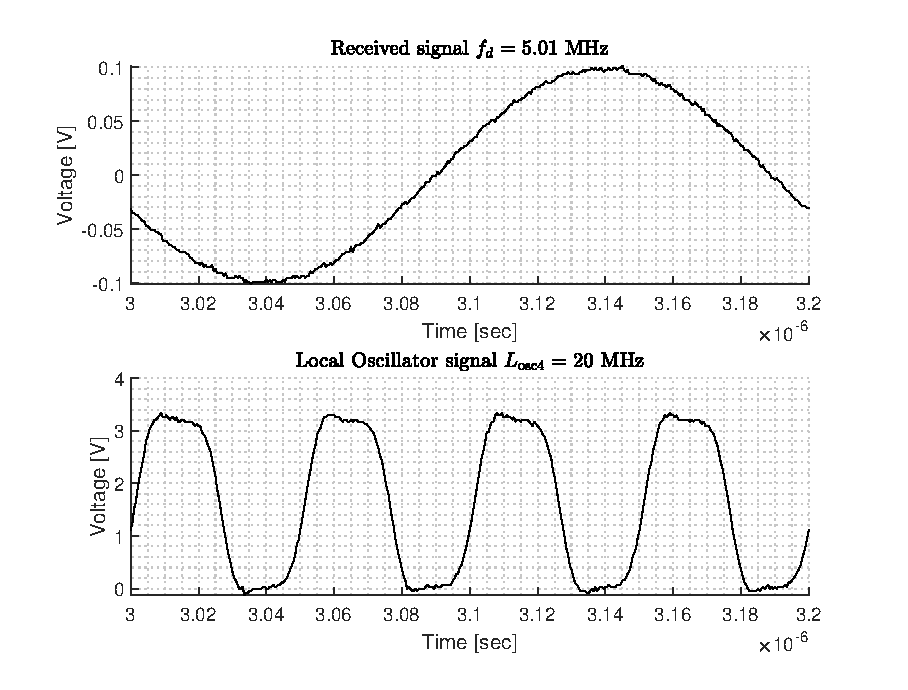
\includegraphics[width=.8\textwidth]{Figures/4_demod_pcb_in.eps}
	\caption[Measured input of demodulator PCB]{Measured input of demodulator PCB (Above) Input from received signal (Below) Input from local oscillator ($f_{0}\cdot4$)}
	\label{fig:4_demod_in}
\end{figure}
\begin{figure}[htbp]
	\centering
	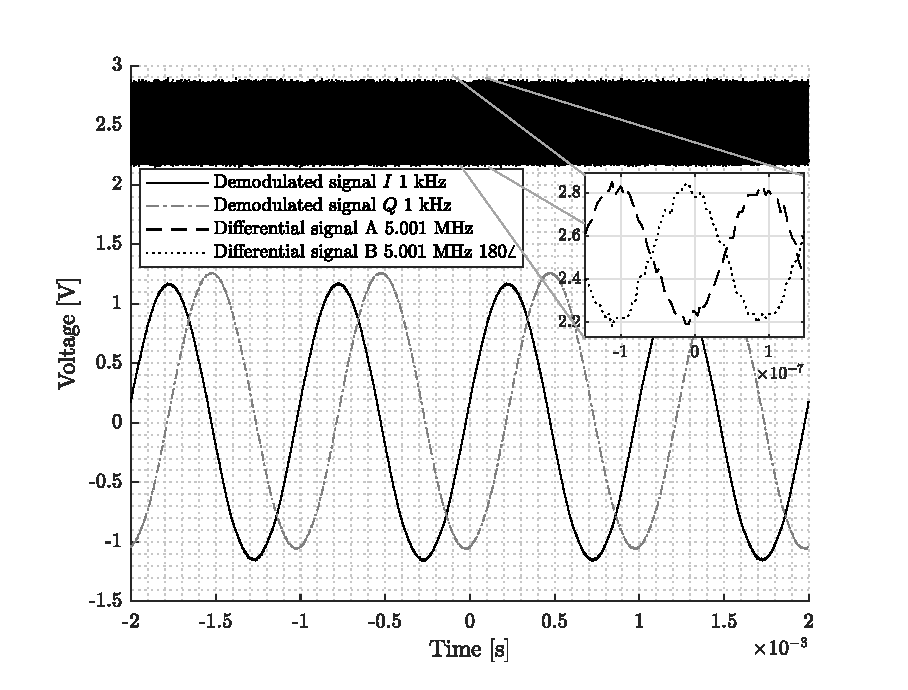
\includegraphics[width=.8\textwidth]{Figures/4_demod_pcb_out.eps}
	\caption[Measured output of demodulator PCB]{Measured output of demodulator PCB}
	\label{fig:4_demod_out}
\end{figure}
The entire schematic of the demodulator can be found in the appendix in \cref{fig:appendix_ad8333}.
\section{Sample and Hold}
After each demodulated burst is sampled, between each sample line pulse repetition it is desired to hold the voltage, so the analogue-to-digital conversion that may be running asynchronously does not sample zero-values between the bursts. Therefore, an experiment is conducted with the sample-and-hold amplifier to verify the functionality. A low-frequency I-Q simulated signal is created from the function generator with a sample gating pulse train to control the sample-and-hold function. Seen in \cref{fig:4_sample_hold_pcb} is the measured inputs and outputs of the circuit during the experiment. Above is the I-Q input and in the middle is the sample gating, and below is the output signal. On the output signal, it is noted the corresponding voltage transients for every pulse in the gate input.
\begin{figure}[htbp]
	\centering
	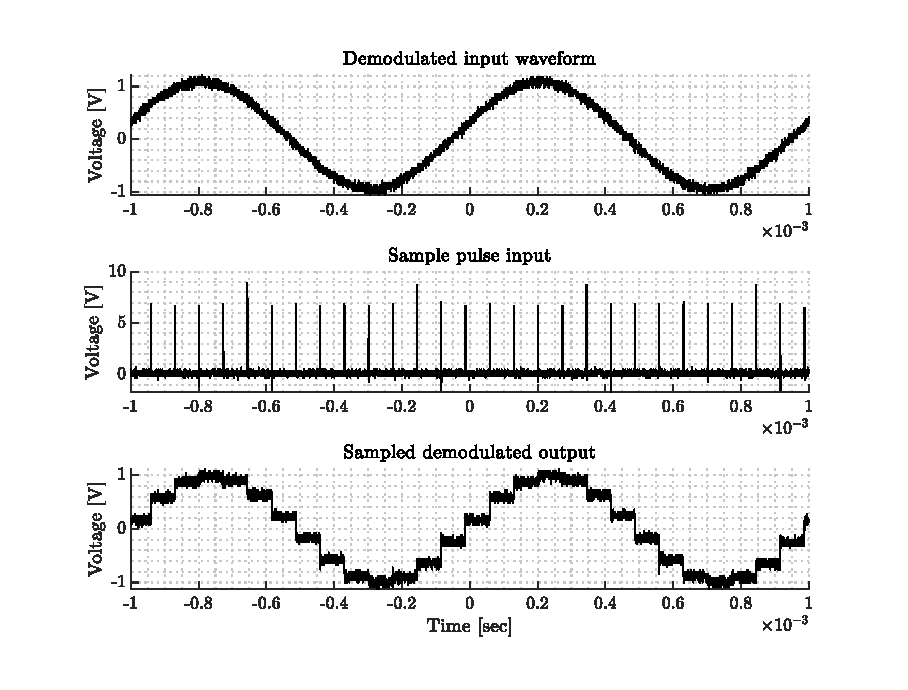
\includegraphics[width=.8\textwidth]{Figures/4_sampler_pcb.eps}
	\caption{Measured input and output of Sample and Hold amplifier}
	\label{fig:4_sample_hold_pcb}
\end{figure}

\section{Pulse-Repetition and Wall Filter}
\section{Digital Signal Processor}


%\begin{figure}[H]
%	\centering
%	\begin{circuitikz}[american voltages]
%		\draw
%		(0,0) to [short, *-] (6,0)
%		to [V, l_=$\mathrm{j}{\omega}_m \underline{\psi}^s_R$] (6,2)
%		to [R, l_=$R_R$] (6,4)
%		to [short, i_=$\underline{i}^s_R$] (5,4)
%		(0,0) to [open, v^>=$\underline{u}^s_s$] (0,4)
%		to [short, *- ,i=$\underline{i}^s_s$] (1,4)
%		to [R, l=$R_s$] (3,4)
%		to [L, l=$L_{\sigma}$] (5,4)
%		to [short, i_=$\underline{i}^s_M$] (5,3)
%		to [L, l_=$L_M$] (5,0);
%	\end{circuitikz}
%	\caption{The nodes short, V, R and L are presented here, but there a lot more}
%	\label{fig:circuitikz}
%\end{figure}
%
%\section{Listings (code)}
%
%\Cref{lst:helloworld} is a nicely formatted block of code. A listing will automatically continue on the next page if it encounters a page break. Many different programming languages can be highlighted. Check the \texttt{listings} package documentation for a list of supported programming languages.

%\begin{listing}[htbp]
%\begin{mintedc}
%#include <stdio.h>
%int main()
%{
%	printf("Hello, World!"); /*printf() outputs the quoted string*/
%	if (n == 0 || n == 1){
%		return n;
%	}
%	j = 0;
%	for (i = 0; i < n-1; i++){
%		if (arr[i] != arr[i+1]){
%			arr[j] = arr[i];
%			j++;
%		}
%	}
%	arr[j++] = arr[n-1];
%	return 0;
%}
%\end{mintedc}
%	\caption{Hello world in C}
%	\label{lst:helloworld}
%\end{listing}



